\DiaryEntry{Virus Outbreak}{2020-03-11}{Maths}

We consider a model where every infected person infects several other (healthy) persons. Let $N(t)$ be the number of infected persons at time $t$; therefore the growth rate of $N(t)$ is proportional to $N(t)$,

\bee
\frac{d N(t)}{dt} = c N(t)
\eee

This is nice and simple; in addition it has a closed-form solution which is easy,

\bee
N(t) = N_0 e^{ct}
\eee

where $N_0 = N(t=0)$ is the initial number of infected persons at time $t=0$. The model is overly simple in that it assumes that there are always healthy persons which can be infected. Implicitely, this assumes that the population is very big (infinite).

A more realistic model is to decrease the infection growth with growing infection rate. A simple model for this

\bee
\frac{d N(t)}{dt} = c(1-\frac{N(t)}{N_\infty} N(t)
\eee

The closer $N(t)$ comes to $N_\infty$, the lower the growth rate is, and therefore the slower $N(t)$ increases. However, the growth rate is positive until it equals $N_\infty$; therefore $\lim_{t \rightarrow \infty} N(t) = N_\infty$. The following plot shows $N(t)$ (blue) and $dN(t)/dt$ (red) with $N_\infty = 2, c = 1$.

\begin{figure}[H]
\centering
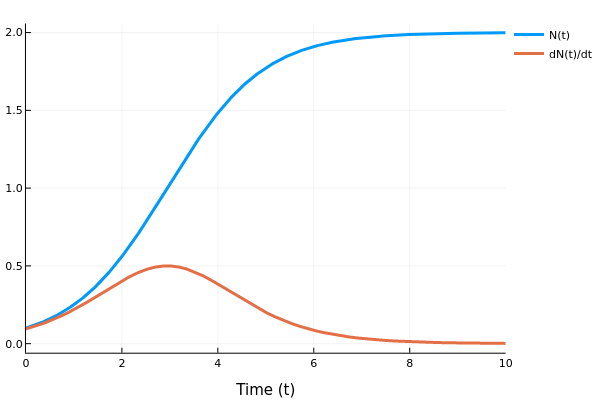
\includegraphics[scale=0.55]{images/virus_1.png}
\end{figure}




%%% Local Variables:
%%% mode: latex
%%% TeX-master: "journal"
%%% End:
